\documentclass[12pt]{article}
\usepackage[margin=0.9in]{geometry} 
\usepackage[utf8]{inputenc}
\usepackage{amsmath}
\usepackage{amsfonts}
\usepackage{amssymb}
\usepackage{graphicx}
\usepackage{color}
\usepackage{float}
\usepackage{scrextend}
\usepackage{enumitem}
\usepackage{parskip}
\usepackage{siunitx}
%\usepackage{listings}

%ignore \hbox issue
\hfuzz=100pt

% title declarations
\newcommand{\doctitle}{Project 4 - NAND3 Simulation \& Layout}
\newcommand{\docsubtitle}{Simulation and Layout Problems}
\newcommand{\docsubsub}{Width = $\SI{0.875}{\mu m}$, Length = $\SI{2.085}{\mu m}$\\ Area = $\SI{1.8244}{\mu m^2}$ Delay = $\SI{59.3223}{ps}$\\ Area * Delay = $\SI{108.226}{}$ }

\renewcommand{\maketitle} {
    \setlength{\parindent}{0pt}
    \begin{center} \
        % top spacing
        \vspace*{1in}

        % main title
        \huge{\doctitle}\\
        %\Large{\docsubtitle}\\
        \large{\docsubsub}

        % naming
        \vspace*{0.2in}
        \large{
            Arthur Hsueh\\
            21582168\\
            UBC - ELEC 402
        }
    \end{center}
}

\begin{document}
\maketitle
\thispagestyle{empty}
\pagebreak

\tableofcontents
\thispagestyle{empty}
\pagebreak

\listoffigures
\thispagestyle{empty}

\listoftables
\thispagestyle{empty}

\pagebreak
\setcounter{page}{1}
\section{MAIN PORTION: NAND3 Simulation \& Layout}
\subsection{NAND3 Gate Design and Layout} % this section shows the layout with rules and dimensions, label pins
\subsubsection{Gate Design}
The first thing for the gate design is to make the schematic for the gate. For a NAND gate, the pull down network is a set of 3 series NMOS transistors, and for the pull up network is a set of 3 parallel NMOS transistors. The inputs are labelled simply as A, B and C. Below is the schematic done in Cadence.
\begin{figure} [H]
    \centering
    \makebox[\textwidth]{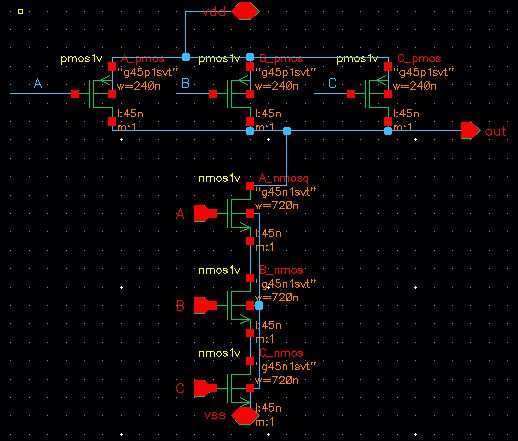
\includegraphics[scale=0.7]{../images/q1_schematic.jpg}}
    \caption{Schematic for the NAND3 Gate}
\end{figure}
For sizing, we initialy sized to an ideal inverter, with PMOS at 2W and NMOS at 3W. This ratio yielded a $t_{pHL}$ that was too large compared to $t_{pLH}$, so the NMOS width needed to be adjusted. Eventually the best case was 6W for the NMOS.
\subsubsection{Gate Layout}
Below is the image of the layout for the NAND3 Gate.
\begin{figure} [H]
    \centering
    \makebox[\textwidth]{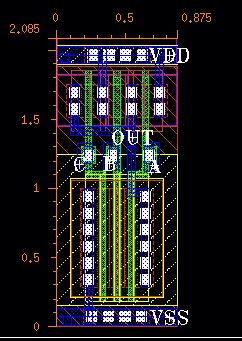
\includegraphics[scale=1.2
    ]{../images/q1_layout.jpg}}
    \caption{Layout for the NAND3 Gate}
\end{figure}
The dimensions and area of the layout are thus shown in the table below
\begin{table} [H]
    \centering
    \begin{tabular}{ccc}
        Width & Length &  Area\\
        \hline
        $\SI{0.875}{\mu m}$ & $\SI{2.085}{\mu m}$ & $\SI{1.8244}{\mu m^2}$
    \end{tabular}
    \caption{Dimensions of the NAND3 Gate}
\end{table}
\subsection{$t_{pHL}$ and $t_{pLH}$ of the gate} %showing tphl and tplh, pattern fo worst-case delay
After extracting parasitics of the gate using PVS-QRC, the gate was simulated to find the delay. The result is shown in the figure below.
\begin{figure} [H]
    \centering
    \makebox[\textwidth]{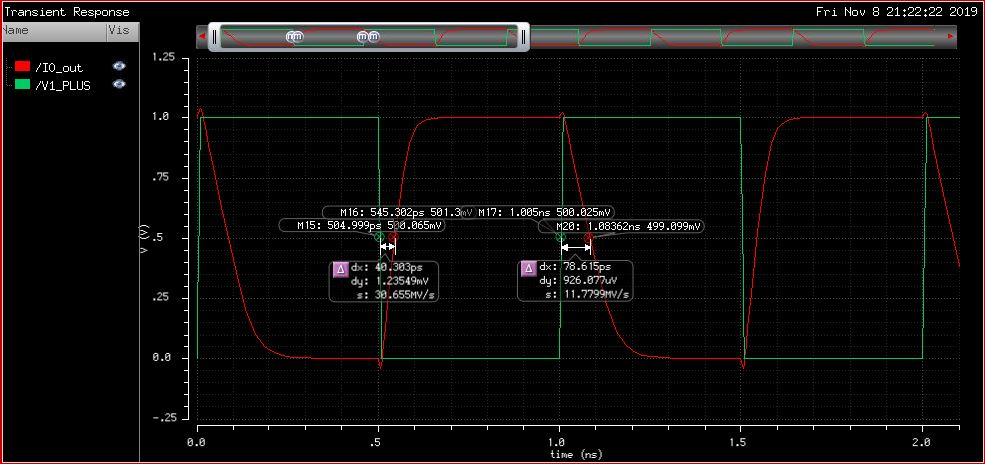
\includegraphics[scale=0.7]{../images/q1_delay.jpg}}
    \caption{Delay Waveform for the NAND3 Gate}
\end{figure}
The delay values are thus shown in table below.
\begin{table} [H]
    \centering
    \begin{tabular}{ccc}
        $t_{pLH}$ & $t_{pHL}$ &  $t_{pd}$\\
        \hline
        $\SI{40.3030}{ps}$&$\SI{78.615}{ps}$ & $\SI{59.3223}{ps}$
    \end{tabular}
    \caption{Delay values of the NAND3 Gate}
\end{table}
I was unable to get the time difference between 5ps, have redone my layout 30-40 times over the course of two weeks. 
\subsection{Worst-case delay}
Analyzing the nature of the circuit, the worst case delay occurs with the following switching pattern.
\[ABC = 110 \rightarrow ABC = 111\]
The worst case occurs when the A and B NMOS are charged, and then C is switched on. This requires the pull down network to fully discharge the stored capacitance in A and B to pull the output fully down to logic 0.
\pagebreak
\subsection{Parasitics}
Below is the original NAN3 schematic with the new parasitics included.
\begin{figure} [H]
    \centering
    \makebox[\textwidth]{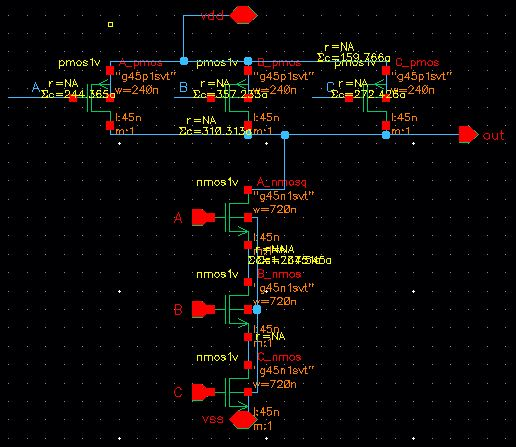
\includegraphics[scale=0.9]{../images/q1_schematic_p.jpg}}
    \caption{Schematic with parasitics for the NAND3 Gate}
\end{figure}
For clarity, the list of parasitics of all nets are shown below.
\begin{figure} [H]
    \centering
    \makebox[\textwidth]{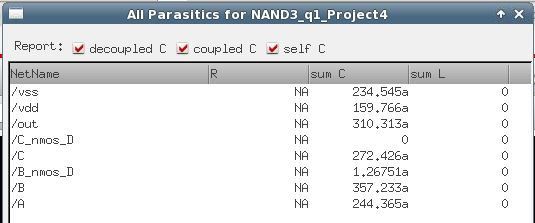
\includegraphics[scale=0.9]{../images/q1_parasitics.jpg}}
    \caption{Parasitics of all nets of the NAND3 Gate}
\end{figure}
\subsection{Inclusion of the 10fF load capacitor}
Below is the testbench circuit used to simulate the NAND3 Gate. As required in the assignment, the output is connected to a $\SI{10}{fF}$ capacitor.
\begin{figure} [H]
    \centering
    \makebox[\textwidth]{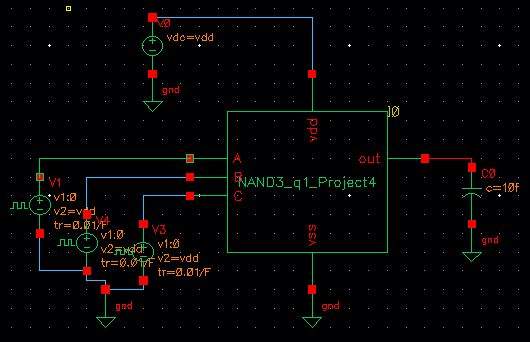
\includegraphics[scale=0.9]{../images/q1_tb_schematic.jpg}}
    \caption{Parasitics of all nets of the NAND3 Gate}
\end{figure}
\pagebreak

\section{Examining the Unknown Circuit}
\subsection{Logic Function of the Block}
To obtain the Boolean expression of the circuit, we look at the pull-down NMOS network to get the dual expression.
Parallel transistors are OR, and series transistos are AND. To find the original boolean expression we simply take the dual 
of the dual function
\[\overline{Y} = (A+B)CD \]
\[\overline{\overline{Y}} = \overline{(A+B)CD} \]
\[Y = \overline{A+B} + \overline{C} + \overline{D} \]
\[Y = \overline{A}\overline{B} + \overline{C} + \overline{D} \]
\subsection{Sizing the gates}
To size the gates we simply need to examine the branches of both the pull-up and pull-down networks.
Parallel connections can apply symmetry properties. 
\begin{table} [H]
    \centering
    \begin{tabular} {c|cc}
        &NMOS W/L&PMOS W/L\\
        \hline
        A&12$\lambda$&16$\lambda$\\
        B&12$\lambda$&16$\lambda$\\
        C&12$\lambda$&8$\lambda$\\
        D&12$\lambda$&8$\lambda$\\
    \end{tabular}
    \caption{Sizings of the Unknown circuits W/L}
\end{table}
\subsection{Worst case input patterns}
For $t_{pHL}$ we want to examine the NMOS network as it is the one that pulls the output from high to low.
We want to find the case where it will take the longeset for all NMOS transistors to discharge any capacitance.
The input pattern is shown below
\[ABCD = 1110 \rightarrow ABCD = 1111\]
If ABC are all on initially, their capacitance is fully charged and turning on the D NMOS will require the pull-down network
to discharge 3 transistors worth of capacitance.

For $t_{pLH}$ we want to examine the PMOS network as it is the one that pulls the output from low to high.
We want to find the case where it will take the longest for all PMOS transistors to charge up capacitance.
The input pattern is shown below
\[ABCD = 1111 \rightarrow ABCD = 0011\]
C and D must off initially; the only case for a longer charge time would be with the A and B PMOS. If A and B are intially turned off
and then turned on, $V_{DD}$ will need to charge up 2 transistors worth of capcaitance.

\pagebreak
\subsubsection{Cadence Simulation Verification}
Below is the schematic for the circuit made in cadence.
\begin{figure} [H]
    \centering
    \makebox[\textwidth]{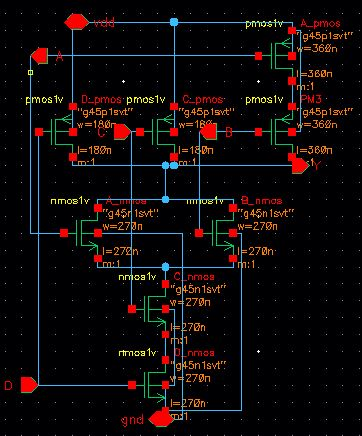
\includegraphics[scale=0.7]{../images/q2_schematic.jpg}}
    \caption{Schematic for the unknown circuit}
\end{figure}
To simulate the $t_{pHL}$, the inputs that don't switch use a vdc source as an input, and for the inputs that do switch, 
we use a vpulse source. 
The simulation schematic for $t_{pHL}$ is shown below
\begin{figure} [H]
    \centering
    \makebox[\textwidth]{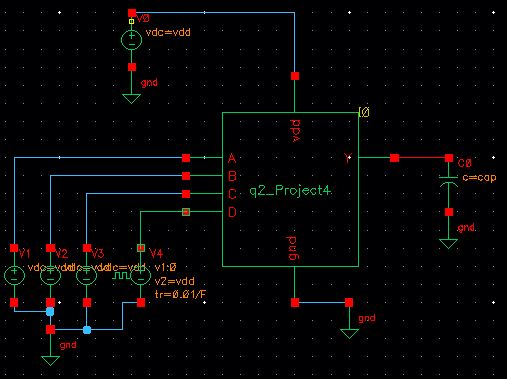
\includegraphics[scale=0.7]{../images/q2_tphl_schematic.jpg}}
    \caption{Schematic for $t_{pHL}$ of the unknown circuit}
\end{figure}
Below is the resulting waveform from simulation.
\begin{figure} [H]
    \centering
    \makebox[\textwidth]{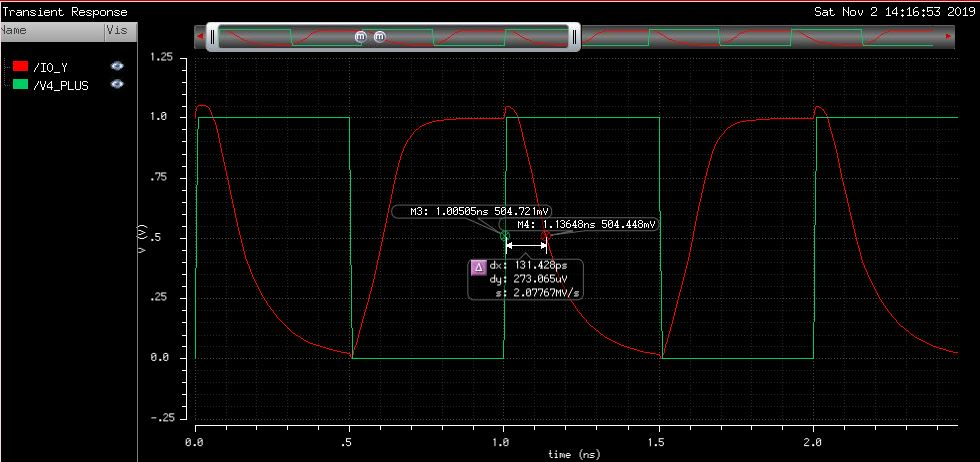
\includegraphics[scale=0.7]{../images/q2_tphl_waveform.jpg}}
    \caption{Waveform for $t_{pHL}$ of the unknown circuit}
\end{figure}

To simulate the $t_{pLH}$, the inputs that don't switch use a vdc source as an input, and for the inputs that do switch, 
we use a vpulse source. 
The simulation schematic for $t_{pLH}$ is shown below
\begin{figure} [H]
    \centering
    \makebox[\textwidth]{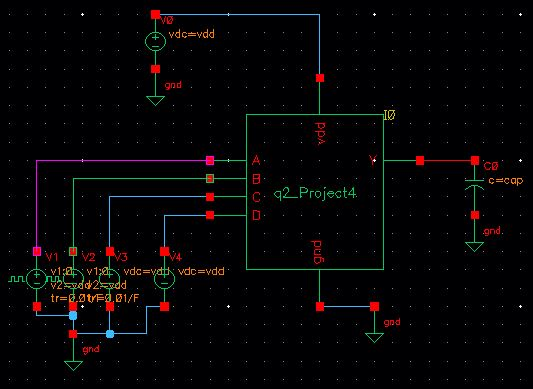
\includegraphics[scale=0.7]{../images/q2_tplh_schematic.jpg}}
    \caption{Schematic for $t_{pLH}$ of the unknown circuit}
\end{figure}
Below is the resulting waveform from simulation.
\begin{figure} [H]
    \centering
    \makebox[\textwidth]{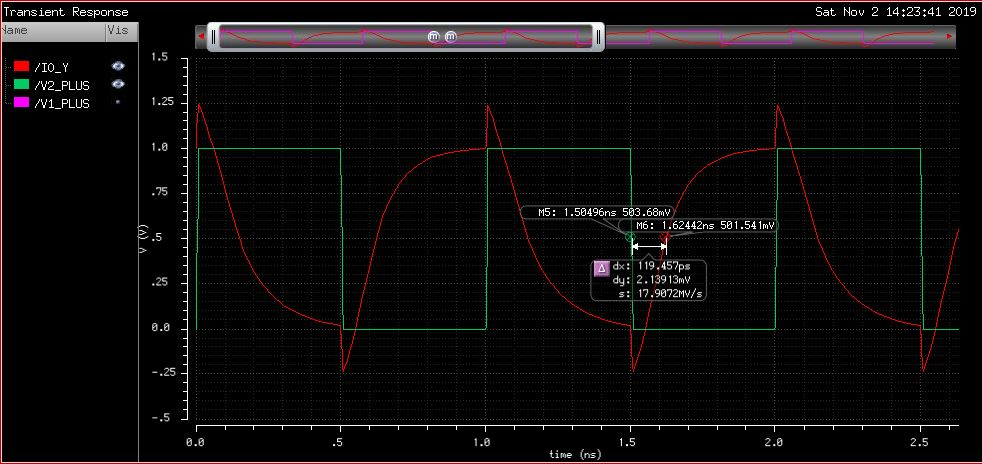
\includegraphics[scale=0.7]{../images/q2_tplh_waveform.jpg}}
    \caption{Waveform for $t_{pLH}$ of the unknown circuit}
\end{figure}

The values of $t_{pHL}$ and $t_{pLH}$ are shown in the table below, based on the measured values from the waveforms.
\begin{table} [H]
    \centering
    \begin{tabular} {cc}
        $t_{pHL}$ & $t_{pLH}$ \\
        \hline
        131.428ps & 119.457ps
    \end{tabular}
    \caption{$t_{pHL}$ and $t_{pLH}$ values of the unknown circuit}
\end{table}
\pagebreak


\section{Examining Figure 1}
\subsection{Output Function Expression}
From the schematic we can see that the transmission gate only passes A when sel is high, and only passes B when selB is high. Thus
the output funciton of the schematic is.
\[OUT = Bselb + A\overline{selb} \]
\subsection{Equivalent RC circuit model}
Below is the image of the equivalent RC circuit model for the path from A to C. 
\begin{figure} [H]
    \centering 
    \makebox[\textwidth]{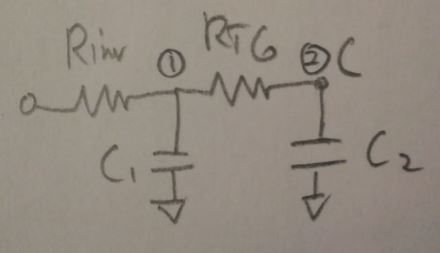
\includegraphics[scale=0.8]{../images/q3b_rc_circuit.jpg}}
    \caption{Equivalent RC circuit of Figure 1}
\end{figure}
There are three main nodes in the circuit path of A to C: the input node(A), the intermediate node between the input inverter and transmission gate(\textcircled{1}), and the node between the transmission gate and the output inverter (C or \textcircled{2}). The contributions at each node are given by the table below.
\begin{table} [H]
    \centering
    \begin{tabular} {ccc}
         & Node \textcircled{1} & Node \textcircled{2}\\
        \hline
        Resistance & $R_{inv}$ & $R_{inv} + R_{TG}$\\
        Capaitance & $C_1$ & $C_2$
    \end{tabular}
    \caption{Resistance and Capacitance contirbutions for the AC path}
\end{table}
\subsection{Delay expression from $A$ to $C$}
From the theory described in class, we note that we can approximate $R_{inv}$ and $R_{TG}$ to use the value of $R_{eqn}$ for an NMOS. The capcitances $C_1$ and $C_2$ have contributions from either input/output devices at the node. They are described in the table below.
\begin{table} [H]
    \centering
    \begin{tabular} {ccc}
         & Node \textcircled{1} - $C_1$ & Node \textcircled{2} - $C_2$\\
        \hline
        General & $C_{eff-inv} + C_{g-TG} + C_{eff-TG}$ & $C_{g-TG} + 2*C_{eff-TG} + C_{g-inv}$\\
        Numerical Expression & $3C_{eff}W + C_gW + 2C_{eff}W$ & $C_gW + 2C_{eff}W + 3C_{eff}W$
    \end{tabular}
    \caption{Capactiance expressions for the RC circuit model of the AC path}
\end{table}
Using Elmore delay, the expression for the delay from A to C is given by
\[t_{AC} = R_{inv}C_1 + (R_{inv} + R_{TG})C_2\]
Substituting in the previous declared values and simplifying yields the delay expression
\[t_{AC} = R(13C_{eff}W + 3C_gW + 6C_gfW) \]
where $R = R_{eqn}\frac{L}{W}$
\subsection{Delay expression through the output}
For the output inverter, we keep the value of $R$ but the capcitance is different. The delay through the output includes $C_{eff}$ of the inverter and the load capacitance $C_{load]}$. This inverter is sized differently, with the multiplier of $f$. The value $f$ reduces the overall resistance becuase of its effect on the width and increases $C_{eff}$. 
\[R \rightarrow \frac{R}{f} \quad and \quad C = 3C_{eff}fW + \SI{50}{fF} \]
Becuase we are taking the RC delay, we take into account that the output inverter expects a step input in the most ideal case, so we need to include the $ln2@$ value in the expression.
\[t_{out} = 0.69 \frac{R}{f}(3C_{eff}fW + \SI{50}{fF}) \]
\subsection{Determining optimal size of the output inverter}
The total delay from A to OUT is thus.
\[t_{total} = t_{AC} + t_{OUT} \] 
\[t_{total} = R(13C_{eff}W + 3C_gW + 6C_gfW) +  0.69 \frac{R}{f}(3C_{eff}fW + \SI{50}{fF}) \]
In order to minimize $t_{total}$ with respect to $f$, we can take the derivative with repsect to $f$ and equate to zero.
\[\frac{dt_{total}}{df} = 6RC_gW - \frac{R*0.69*\SI{50}{fF}}{f^2} = 0 \]
Solving for f
\[ f = \sqrt{\frac{0.69*\SI{50}{fF}}{6C_gW}}\]
Taking the value of $C_g = \SI{2}{fF/\mu m}$ and $W = W_n = \SI{0.4}{\mu m}$, the value of $f$ is.
\[f = 2.68 \sim 3 \]
\end{document}  